% Preamble
% =============================================================================

% Class of the document.
\documentclass[12pt,a4paper]{article}
% article : short article.
% report  : mid-length report.
% book    : book or thesis redaction.

% Paragraph skip length (default to 0).
\setlength{\parskip}{1ex}

% Packages
% =============================================================================

% Encoding
% -----------------------------------------------------------------------------

% Babel.
\usepackage[french]{babel}
% FontEnc.
\usepackage[T1]{fontenc}
% InputEnc.
\usepackage[utf8]{inputenc}

% Define \escapeus command to escape underscores.
\makeatletter
\DeclareRobustCommand*{\escapeus}[1]{
    \begingroup\@activeus\scantokens{#1\endinput}\endgroup}
\begingroup\lccode`\~=`\_\relax
    \lowercase{\endgroup\def\@activeus{\catcode`\_=\active \let~\_}}
\makeatother

% Text
% -----------------------------------------------------------------------------

% Acronym.
\usepackage{acronym}
% CsQuote.
\usepackage[style=french,french=guillemets]{csquotes}
% Enumerate.
\usepackage{enumerate}
% HyperRef.
\usepackage[hyperfootnotes=false,hidelinks]{hyperref}
% URL.
\usepackage{url}

% Algorithms
% -----------------------------------------------------------------------------

% Algorithm2E.
\usepackage[french,onelanguage,linesnumbered,ruled,vlined,commentsnumbered]{algorithm2e}

% Source code
% -----------------------------------------------------------------------------

% Listings.
\usepackage{listings}
% Minted.
\usepackage{minted}
% Caption.
\usepackage{caption}
\newenvironment{code}{\captionsetup{type=listing}}{}

% Files
% -----------------------------------------------------------------------------

% FancyVRB.
\usepackage{fancyvrb}
% Redefine \VerbatimInput.
\RecustomVerbatimCommand{\VerbatimInput}{VerbatimInput}
{
    fontsize=\footnotesize,
    frame=lines,         % Top and bottom rule only.
    framesep=1.5em,      % Separation between frame and text.
    rulecolor=\color{red!50!green!50!blue!50!},
    labelposition=topline,
    commandchars=\|\(\), % Escape character and argument delimiters for commands within the verbatim.
    commentchar=*        % Comment character.
}

% Figures
% -----------------------------------------------------------------------------

% GraphicX.
\usepackage{graphicx}
% SVG.
\usepackage{svg}
% WrapFig.
\usepackage{wrapfig}

% Charts
% -----------------------------------------------------------------------------

% PGFPLots
\usepackage{pgfplots}
\pgfplotsset{compat=1.16}
\usepgfplotslibrary{units}

% Mathematics
% -----------------------------------------------------------------------------

% AmsFonts.
\usepackage{amsfonts}
% AmsMath.
\usepackage{amsmath}
% AmsText.
\usepackage{amstext}
% AmsThm.
\usepackage{amsthm}
\newtheorem{prr}{Propriété}
\newtheorem{pro}{Proposition}
\newtheorem{thm}{Théorème}
\newtheorem{lem}{Lemme}
% NumPrint.
\usepackage{numprint}

% Physics
% -----------------------------------------------------------------------------

% Physics.
\usepackage{physics}

% Presentation
% -----------------------------------------------------------------------------

% XColor.
\usepackage{xcolor}

% References
% -----------------------------------------------------------------------------

% CleveRef.
\usepackage{cleveref}

% Structure.
% -----------------------------------------------------------------------------

% Geometry.
\usepackage{geometry}
% PDFLScape.
\usepackage{pdflscape}
% MultiCol.
\usepackage{multicol}
% TitleSec.
\usepackage{titlesec}
\newcommand{\sectionbreak}{\clearpage} % Use a page break before new sections.
% VMargin.
\usepackage{vmargin}
% FootMisc.
\usepackage[bottom]{footmisc}

% Symbols
% -----------------------------------------------------------------------------

% SIUnitX.
\usepackage{siunitx}

% Table
% -----------------------------------------------------------------------------

% Array.
\usepackage{array}
% BookTabs.
\usepackage{booktabs}
% CSVSimple.
\usepackage{csvsimple}

% Document
% =============================================================================

\begin{document}

\title{Analyse de performance et optimisation de code}
\author{AYOUB Pierre -- BONNAFOUS Camille -- FLAMANT Océane}

\maketitle

\begin{figure}[b]
    \centering
    
\includegraphics[scale=0.3]{figures/isty.jpg}
\end{figure}

\newpage
\begin{abstract}

La simulation numérique est un procédé informatique visant à modéliser un
phénomène par ordinateur, s'agissant le plus souvent d'un phénomène
physique. Cette modélisation prend forme par des systèmes d'équations
décrivant l'état du système physique représenté à chaque instant. De
nombreux domaines scientifiques convergent vers la simulation
informatique, tel que certaines branches de la physique, de l'analyse
et de l'optimisation mathématique, ou encore le calcul haute
performance en informatique. Enfin, la simulation trouve naturellement
de nombreuses applications concernant des sujets variés, tel que la
simulation du climat et des évènements météorologiques, la simulation
d'essais nucléaires, de l'effet d'un médicament sur un corps, ou encore
des astres et de l'univers. Ce rapport s'articulera donc autour de l'analyse et
de l'optimisation d'un code de calcul, coeur des simulations numériques
présentés ci-dessus.

\end{abstract}

\tableofcontents

\section{Introduction}

Le projet que nous vous présentons aujourd'hui consiste à analyser puis, grâce à
nos mesures, optimiser un code de calcul, appelé kernel. Les mesures doivent
s'effectuer à l'aide de l'instruction \textit{x86} \textit{RDTSC}, et des deux
outils d'analyse de performance suivant : \textit{MAQAO} et \textit{LIKWID}.
\textit{RDTSC} nous permet de mesurer le nombre de cycle entre deux instants,
\textit{MAQAO} rends possible l'exécution d'analyses statiques (\textit{CQA}) et
dynamiques (\textit{LPROF}) d'un binaire, présentées par un rapport haut niveau
à l'aide de \textit{ONE-VIEW}, enfin \textit{LIKWID} permet d'obtenir un grand
nombre de métriques très précises concernant, notamment, l'usage de la mémoire.

Afin d'étudier les différents niveaux de la hiérarchie mémoire, chaque membre du
groupe analysera un niveau qu'il se verra assigné. Ci-dessous la liste des
assignatons :
\begin{description}

    \item[Pierre] Cache L1 : 
        \begin{itemize}
            \item Intel Core i7-6600U
            \item 32 kiB L1i, 32 kiB L1d
            \item 256 kiB L2
        \end{itemize}
    \item[Océne ] Cache L2 : 
        \begin{itemize}
            \item Cache L1 : 32K
            \item Cache L2 : 256K
            \item Fréquence 2,40GHz
        \end{itemize}
    \item[Camille] RAM : 
        \begin{itemize}
            \item TO DO
        \end{itemize}
\end{description} 

Le déroulement du projet s'est effectué en plusieurs étapes distinctes :
\begin{description}
    \item[Analyse du code] Cette phase consiste à analyser le programme d'un
        point de vue d'architecture informatique. Il convient d'étudier les
        choix mis en œuvres afin d'implémenter le ou les calculs nécessaires.
    \item[Protocole expérimental] Une fois l'analyse effectuée, nous
        pouvons en déduire le moyen le plus adapté afin de mesurer les
        performances de notre implémentation. Nous allons donc mettre en
        avant les critères théoriques à atteindre dans nos mesures, puis
        nous exposerons la manière dont nous avons mis ceci en pratique.
    \item[Optimisations et mesures] Grâce au protocole mis en place, nous
        pouvons quantifier la performance du programme. De ce fait, nous serons
        en mesure d'expérimenter différentes techniques d'optimisation sur le
        programme et d'en calculer l'accélération.
\end{description}

\section{Analyse du code}

Présentons notre kernel par son prototype, que nous observons sur le
Listing~\ref{lst.baseline.noopt.prot} Nous voyons que 3 variables manipulées :
\begin{itemize}
    \item $n$ correspond à la taille de nos tableaux.
    \item $a$ est un tableau de \textit{float} à deux dimensions dont la taille
        en fonction de $n$ : $4n^2$ Bytes.
    \item $b$ est un tableau de \textit{double} à une dimension dont la taille
        en fonction de $n$ : $8n$ Bytes.
\end{itemize}

\begin{listing}[h]
    \begin{minted}[linenos,numbersep=5pt,frame=lines,framesep=2mm]{C}
void baseline(unsigned n, float a[n][n], double b[n])
    \end{minted}
    \caption{Prototype du kernel non-optimisé}
    \label{lst.baseline.noopt.prot}
\end{listing}

Nous sommes face à un code de calcul très simple en apparence, illustré dans le
Listing~\ref{lst.baseline.noopt} : deux boucles imbriquées, un branchement, un
calcul mêlant multiplication et exponentiel. Plusieurs éléments remarquables qui
risquent de poser problème au niveau de la rapidité d'exécution apparaissent
alors : les boucles impliquent qu'il faut prêter attention au sens de parcours
des tableaux, le branchement nous laisse penser qu'il faudrait essayer de le
supprimer, enfin l'exponentiel et la multiplication sont des opérations lourdes.

\begin{listing}[h]
    \begin{minted}[linenos,numbersep=5pt,frame=lines,framesep=2mm]{C}
for (j = 0; j < n; j++) {
    for (i = 0; i < n; i++) {
        if (j == 0)
            b[i] = 1.0;
        b[i] *= exp(a[i][j]);
    }
}
    \end{minted}
    \caption{Kernel non-optimisé}
    \label{lst.baseline.noopt}
\end{listing}

\section{Protocole expérimental}

La mise en place d'un protocole expérimental de mesure est une étape nécessaire
et cruciale dans tout processus d'optimisation de code. D'une part, le but de ce
protocole est de mettre en lumière les points chauds du programme, c'est-à-dire
les parties du code qui ralentissent considérablement l'exécution des calculs :
ces points chauds seront les cibles de nos optimisations. D'autre part, après
chaque tentative d'optimisation, le protocole doit nous permettre de mesurer
l'impact de cette dernière, qu'il soit positif ou négatif, et enfin de le
quantifier.

\subsection{Théorie}

Lors de nos expériences, de nombreux paramètres peuvent être sujets à des
variables aléatoires ou à l'erreur de mesure, ainsi un résultat peut être
biaiser. Afin d'éviter cela, il est impératif d'utiliser une valeur
représentative de nos différentes mesures : une valeur moyenne ou une valeur
médiane. La valeur médiane semble être un meilleur candidat contrairement à la
moyenne, car cette dernière peut-être fortement modifié par une valeure extrème
qui n'as pas lieu d'être. C'est donc la valeur médiane que nous prendrons des
réslutats de nos mesures successives issues des méta-répétitions.

Pour que chaque membre de l'équipe puisse travailler sur son niveau de mémoire
cache, il nous faut trouver la taille des données d'entrée à utiliser. Selon le
protoype présenté dans le Listing~\ref{lst.baseline.noopt.prot}, la taille
totale de nos données d'entrées est de $4n^2 + 8n$, avec $n$ la taille rentrée
en paramètre du programme.

\subsubsection{Cache L1}

Ci-dessous les paramètres des mesures :
\begin{enumerate}[(1)]
    \item Taille pour tenir dans L1 : $n = 88$.
        En effet, $(n^2 * 4) + (n * 8) = 31680 B$, sachant que la taille du
        cache est de $32 kiB = 2^{15} = 32768 B$, et que si l'on prends $n =
        90$, on obtient $33120 B$, on a bien : $n = 88 < L1 < n = 90$ avec une
        bonne marge de sécurité.
    \item Nombre de répétition du warm-up : 1000. Ce nombre est suffisant pour
        avoir ensuite des mesures stables dans tout nos tests car les caches
        sont remplis avec nos tableaux, choisi par observation.
    \item Nombre de répétition des mesures : on choisi un nombre qui nous permet
        d'avoir à peu près 3 secondes par méta-répétition. Ce nombre vari en
        fonction de la taille de notre tableau. Avoir quelques secondes de
        mesures permet d'avoir une faible marge d'erreur de mesures des cycles
        avec un RDTSC. Par exemple, pour une taille de 89, on peut choisir
        1000000.
\end{enumerate}

\subsubsection{Cache L2}
Pour que les deux tableaux entrent entièrement dans le cache L2, il faut 
que la formule respecte les contraintes suivantes : 
\begin{itemize}
    \item La taille totale doit être plus grande que la taille du cache 
    L1 (1). Pour plus sécurité il a été décidé que la taille totale devait 
    être au moins trois fois plus grande que celle du L1.
    \item L2 partage sa mémoire pour stocker à la fois les instructions, 
    les données et ce qui tourne en background, on ne peut donc en utiliser 
    approximativement que 90\% (2). 
\end{itemize}

Ces deux contraintes peuvent être transformée sous forme d'inéquation :
\begin{itemize}
    \item (1) : $3*TL1 < 4n*n + 8n$,
    \item (2) : $4n*n + 8n \le 0,9*\text{TL2}$
\end{itemize}
Après la résolution de ces équations on obtient $n=156$ comme minimum et $n=242$
comme maximum.

\subsubsection{RAM}

TODO

\subsubsection{Analyse de sensibilité}

Une fois que l'on connait la taille des données à fournie en entrée, 
il faut effectuer une analyse de sensibilité pour les autres paramètres. 
\begin{description}
    \item[Nombre de méta-répétition des mesures] Il nous est donné à 31. C'est
        le nombre donné dans la consigne, qui est suffisant pour avoir un nombre
        de mesure significatives.
    \item[Le nombre de warmup] Il doit se situer entre 1 et 1000. Pour le
        déterminer, il doit être le seul paramètre que l'ont fait varier. On
        fait plusieurs exécutions et, avec les valeurs obtenues, on fait une
        courbe pour voir à partir de quelle valeur cela devient stable. Il faut
        aussi vérifier que
        $\frac{\text{médiane}-\text{minimum}}{\text{minimum}}$ est inférieur à
        5\%. 
    \item[Le nombre de répétitions] On le trouve de la même manière que le
        nombre de warmup.
\end{description}

\subsection{Pratique}

Lors de nos première tentatives pour trouver les paramètres, nous avons remarqué
que ce qui prenait le plus de temps dans notre noyau de calcul était
l'exponentiel. Afin de pouvoir vérifier si nos paramètres sont corrects, nous
avons donc modifié le fichier \textit{kernel.c} pour que ce soit le temps de
récupération des données qui soit le plus grand. Cette version n'est utilisé que
pour tester la véracité des paramètres trouvés dans la section précédente, et
nous pour évaluer les performances des optimisations ou des compilateurs.

\subsubsection{Cache L1}

On peut observer une nette différence de performance entre un $n = 88$ et un $n
= 90$, qui se traduit par le fait de tenir ou de ne pas tenir en cache
\textit{L1}. On assigne le programme de calcul au coeur n°2 de la machine, sur
son numéro de thread physique, dans le but de limiter les changements de
contexte et de flush de la mémoire cache. Enfin, les tests sont effectué en
rescue mode, sans interface graphique, avec le minimum de tâches tournant en
arrière plan.

Tout les mesures effectuées dans le cache L1 sont automatiser par un script
(\textit{bench.sh}). Ce script permet d'aisément exécuter l'ensemble des tests
dans un environement idéal, ainsi que d'assurer la reproductibilité du protocole
expérimental, critère important d'une méthode scientifique.

\subsubsection{Cache L2}

Pour vérifier le calcul théorique de la taille des données j'ai utilisé
likwid-perftcr afin de voir si les données transitaient bien par le cache L2.
Après avoir compilé avec gcc uniquement j'ai exécuté l'exécutable avec likwid et
voici les résultats obtenus :
\newline

\begin{tabular}{|c|c|}
  \hline
  n & Data Volume (GByte) \\
  \hline
  100 & 4,24 \\
  \hline
  150 & 14,06 \\
  \hline
  220 & 37,9 \\
  \hline
  235 & 34,4 \\
  \hline
\end{tabular}

On observe que ces résultats sont en corrélation avec les résultats théoriques
en dessous de 156 pratiquement aucune donnée ne passe par le cache L2 et 
quand on se rapproche de 242 une partie des données ne semble plus passer 
dans L2 je suppose donc que ces données vont directement dans le cache L3.
Au vu de ces informations, j'ai choisi de prendre 220 comme taille de 
données.

Voici, ci-contre le graphique obtenu pour trouver le bon nombre de warmup. On
peut observer que le nombre de cycle semble se stabiliser au alentour de 100
warmup. Pour plus de sécurité j'ai choisit 150 pour le nombre de warmup.

\begin{figure}[h]
    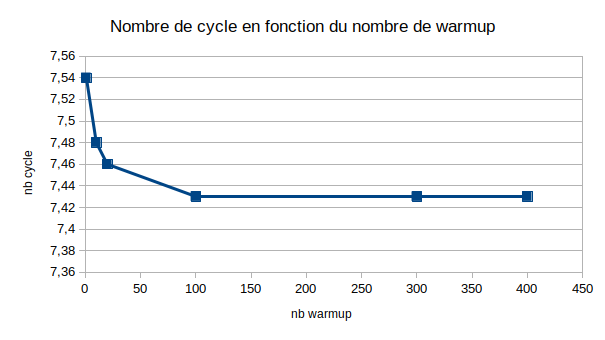
\includegraphics[scale=0.8]{figures/L2/L2warmup.png}
    \caption{Sans l'exponentiel}
\end{figure}

J'ai ensuite vérifié avec le calcul de l'exponetiel et on obtient bien le 
même résultat. 

\begin{figure}[h]
    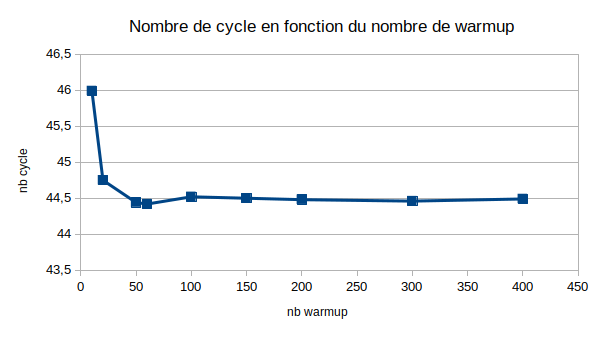
\includegraphics[scale=0.8]{figures/L2/L2warmup2.png}
    \caption{Avec l'exponentiel}
\end{figure}

Pour trouver le bon nombre de répétition j'ai uniquement fait les test avec
l'exponentiel. Comme vous pouvez le voir, on peut remarquer que l'ensemble est
stable, les variations sont minimes. J'ai chosit comme nombre de répétition
1200.
\begin{figure}[h]
    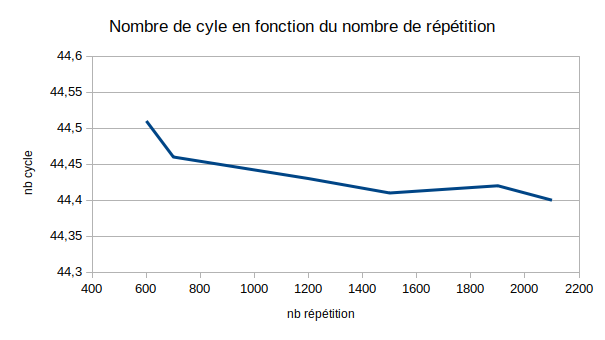
\includegraphics[scale=0.8]{figures/L2/L2repet.png}
    \caption{ }
\end{figure}

\subsubsection{RAM}

TODO

\section{Optimisations et mesures}

Dans cette section, nous présentons les résultats des mesures des différentes
tentatives d'optimisation du code. La phase 1 correspond, pour résumer, à
identifier les points chauds et tester différentes configuration de compilation.
La phase 2 correspond, notamment, à une optimisation active du code en y apportant
des modifications.

\subsection{Phase 1}

\subsubsection{Cache L1}

\subsubsection{Cache L2}

\begin{tabular}{|c|c|c|}
  \hline
	Numéro  & Commande & Résultat\\
  \hline
  1 & gcc -O2 & ?? \\
    \hline
  2 & gcc -O3 & ?? \\
    \hline
  3 & gcc -O3 -march=native & ?? \\
    \hline
  4 & icc -O2 & ?? \\
    \hline
  5 & icc -O3 & ?? \\
    \hline
  6 & icc -O3 -xHost & ?? \\
  \hline
\end{tabular}

\subsubsection{RAM}

TODO

\subsection{Phase 2}

TODO

\section{Conclusion}

TODO

\newpage
\section*{Acronymes}

\begin{acronym}
\end{acronym}

\end{document}
